Unsere Hilfsorganisation möche auf ihrer Homepage eine Liste aller eingegangenen Zahlungen anzeigt.  Schreiben Sie ein XSL Stylsheet, das bei Anwendung auf das XML Dokument folgende Webseite generiert:

\begin{figure}[H]
\centering
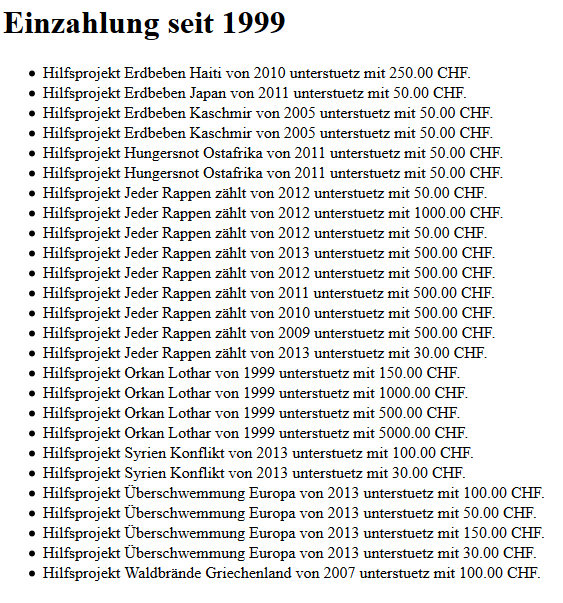
\includegraphics[scale=0.4]{fig/xslt_bootcamp_ziel.png}
\end{figure}


Beachten Sie, dass die Liste alphabetisch nach dem Hilfsprojekt zu sortieren ist. Hier wurde zusätzlich die Jahreszahl beim Sortieren berücksichtigt, dies ist jedoch nicht unbedingt nötig. Der generierte Output muss gültiges XHTML sein. Vervollständigen Sie folgendes XSL Stylesheet.

\lstinputlisting{xslt_bootcamp.xsl}